
\section{Тест производительности}

Для тестов я использвал утилиту gnuplot для построения графиков зависимости времени операций от количества разрядности входных чисел. Так же для сравнения использовал библиотеку int\_width для 128-битных чисел и chrono для замера времени.
  
\begin{alltt}
igor@igor-Aspire-A315-53G:~/Рабочий стол/c++/DA/lab6$ ./a.out
a = 753275733897352885583252657455685685, b = 723587383839

Сложение: 
753275733897352885583253381043069524
Моя реализация: 2.2498e-05
Библиотека <int_width>: 0.00179459

Вычитание: 
753275733897352885583251933868301846
Моя реализация: 4.602e-06
Библиотека <int_width>: 0.000723548

Деление: 
1041029391503263989488349
Моя реализация: 1.76e-05
Библиотека <int_width>: 0.000360422
igor@igor-Aspire-A315-53G:~/Рабочий стол/c++/DA/lab6$
\end{alltt}

Из приведенных тестов видно, что операции сложения, вычитания и деления проходят быстрее. Далее я приведу графики зависимости времени выполнения операций от количества разрядов числа. 
\begin{figure}[h]
  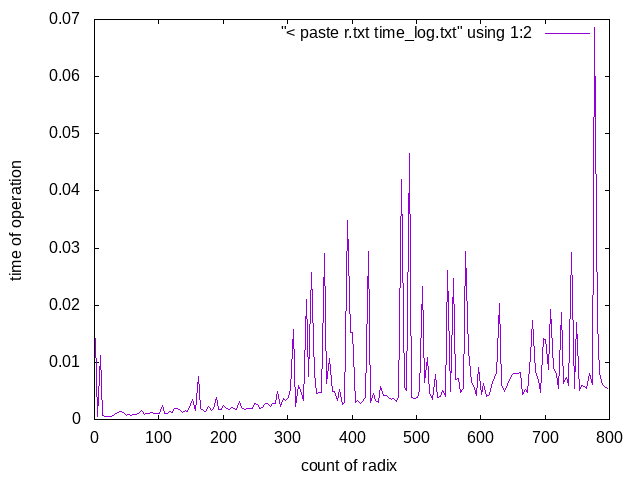
\includegraphics[scale=0.3]{../plots/plus.png}
  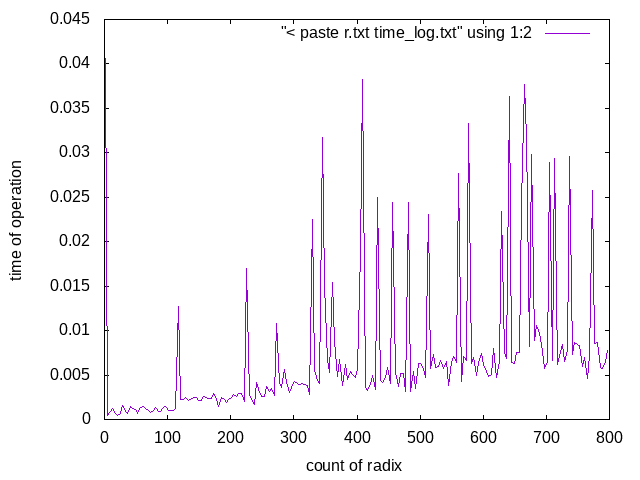
\includegraphics[scale=0.3]{../plots/minus.png}
  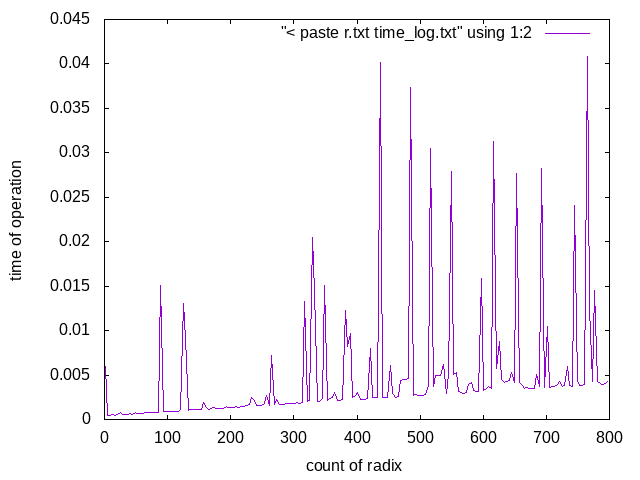
\includegraphics[scale=0.3]{../plots/comp.png}
  \caption{Сложение, вычитание и сравнение}
\end{figure}
\begin{figure}[h]
  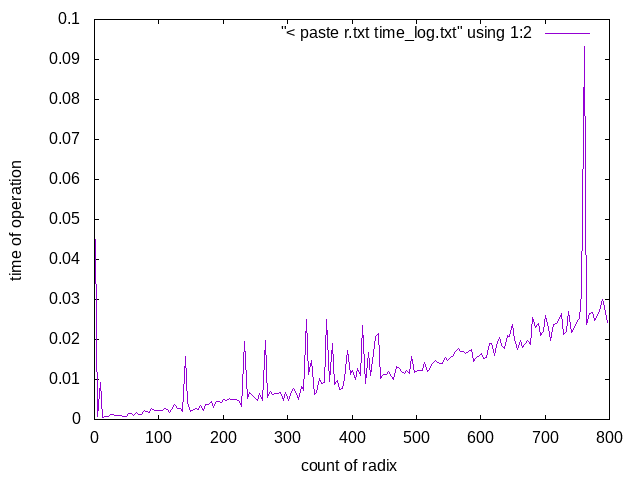
\includegraphics[scale=0.3]{../plots/mul.png}
  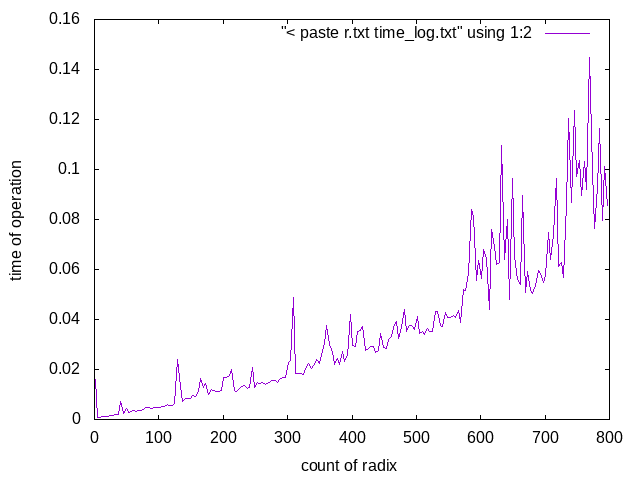
\includegraphics[scale=0.3]{../plots/div.png}
  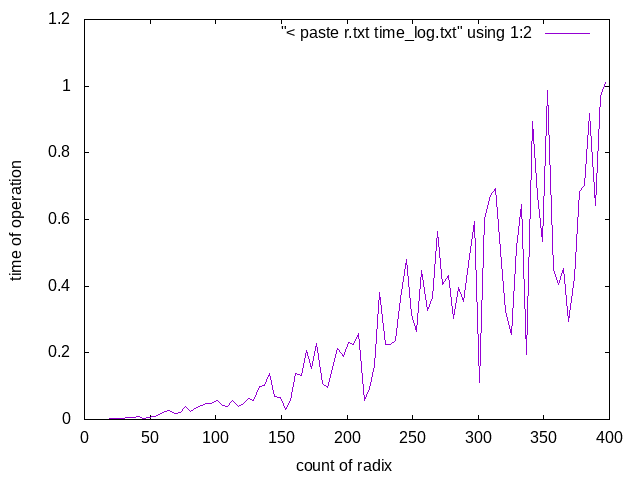
\includegraphics[scale=0.3]{../plots/degree.png}
  \caption{Умножение, деление и возведение в степень}
\end{figure}

\pagebreak
